\section{Problem Formulation}
In this section we present the general concept of our learning approach. The basic idea is to interpret the folded state of a box as a series of rotation angles along each edge, where the problem of predicting folded state is turned into a problem of predicting these angles. 
\subsection{Definitions and Notations}
As an input to our method, we expect a 2D designed layout of a box represented as a flat triangular mesh $L$. As an output of our method, we deform the input triangular mesh into its 3D realization $R$, according to predicted angles along each of its edges.(An example is shown in Figure~\ref{fig:approximation})\\
\begin{figure}
	\centering
	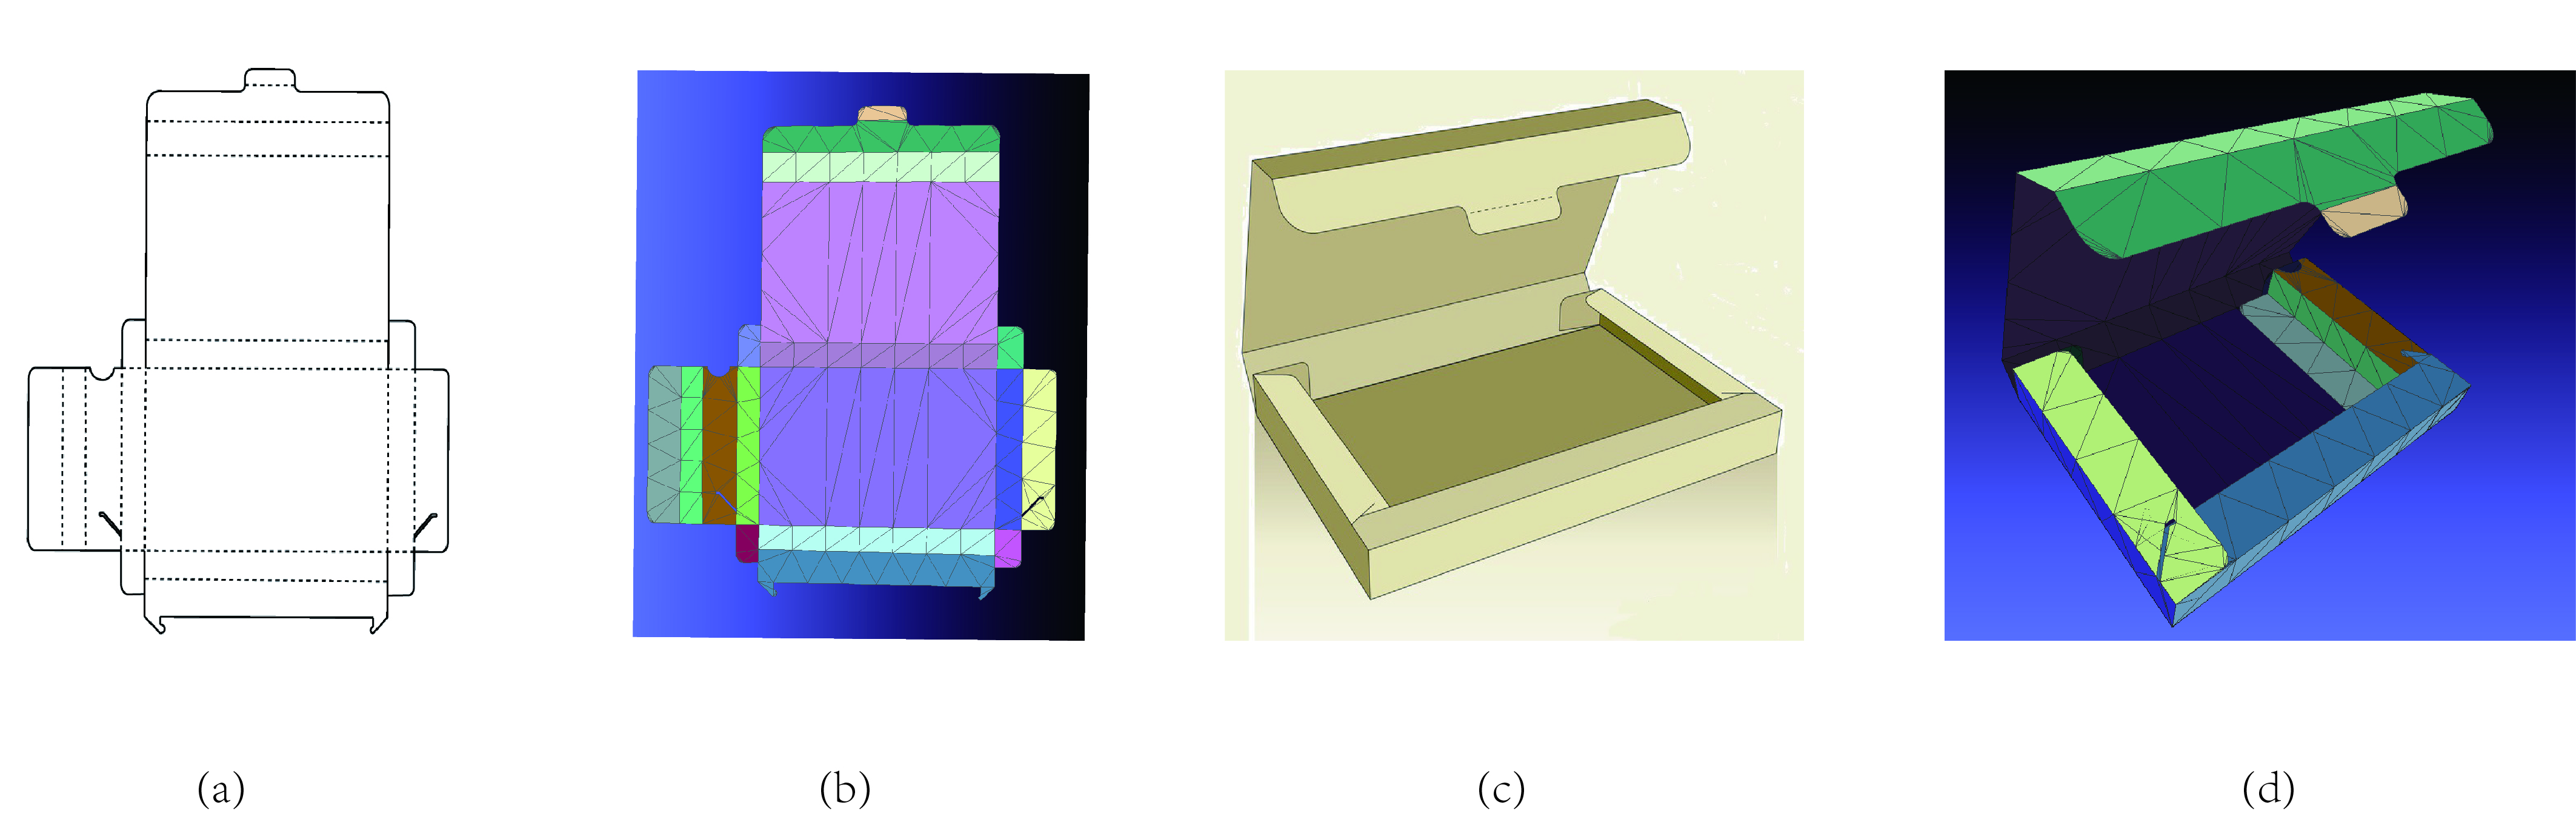
\includegraphics[width=3.0in]{images/approximation.jpg}
	\caption{Given a design layout (a) and its 3D realization (c), we can approximately represent them by triangular mesh as (b) and (d).}
	\label{fig:approximation}
\end{figure}
Without loss of generality, learning to predict the folded state of a box is learning an operator $\mathcal{F}$ that maps every 2D layout to its 3D realization:
\begin{equation}
\mathcal{F}:\{L\}\rightarrow\{R\}
\label{equ:F_0}
\end{equation}
in which $\{L\}$ is the set of all designed layout of boxes represented by 2D triangular meshes and $\{R\}$ is the set of 3D realization of the same boxes represented by deformed triangular meshes. A triangular mesh consists of a set of vertices, edges and faces~$M=(V,E,F)$. The number of vertices, edges and faces varys from one mesh to another. However, a pair of $(L,R)$ as the 2D layout and its correspondent 3D realization share the same topology and therefore has same number of vertices, edges and faces. A flat mesh as a 2D layout from $\{L\}$ has its $z$ component of each vertices set to constant zero: $X_z(v) \equiv 0$ and its normal of each face to $(0,0,1)^T$: $N(e) \equiv (0,0,1)^T$.
\subsection{From Shape Mapping to Functional Mapping}
It is difficult to design a model and a learning scheme to learn the operator in (\ref{equ:F_0}). As we stressed before, the folded state of a box can be represented by a series of rotation angles along each edge which is why we can learn operator $\mathcal{\bar{F}}$ in (\ref{equ:F_1}) instead of $\mathcal{F}$ in (\ref{equ:F_0}):
\begin{equation}
\mathcal{\bar{F}}:\{(X_0,X_1,...,X_n)\}\rightarrow\{\Theta\}
\label{equ:F_1}
\end{equation}
in which the $\{(X_0,X_1,...,X_n)\}$ is a set of feature tensors that is extracted from $\{L\}$ to represent each 2D layout. A feature tensor is composed of n feature functionals and a feature functional has the form of $X_n:E\rightarrow\mathbb{R}$ which is a real value functional that maps each edge of a mesh to a real value. The $\{\Theta\}$ is a set of dihedral angle functionals that maps each edge of a mesh to its angle of folded state. One dihedral angle functional has the form of $\Theta:E\rightarrow [0,2\pi]$. To avoid ambiguity, we define the dihedral angle to be the one that the face normal pointed to.({\color{red} {need more elaberation with the definition of ``positive dihedral angle"}})\\
Unfortunately, it is still difficult to learn the operator $\mathcal{\bar{F}}$, since the dimension number of tensors and functionals in $\{(X_0,X_1,...,X_n)\}$ and $\{\Theta\}$ varies from one pair of $(L,R)$ to another.\\
To cope with this problem, we approximate each functionals as a linear combination of $K$ basis functionals $\Phi = \{\phi_k\}$ as $X_n \approx \sum \alpha_k \phi_k$  and $\Theta \approx \sum \theta_k \phi_k$. Each pair of $(L,R)$ shares the same $\Phi$, which allows us to further change the problem into learning $\mathcal{\hat{F}}$ as a mapping from the feature coefficient tensors to dihedral angle coefficients:
\begin{equation}
\mathcal{\hat{F}}:\{(\{\alpha_k\}_0,\{\alpha_k\}_1,...,\{\alpha_k\}_n)\}\rightarrow\{\{\theta_k\}\}
\label{equ:F_2}
\end{equation}
\subsection{Choice of Basis Functionals}
It is tricky to construct basis functionals $\{\Phi\}$, which are derived from the first $K$ smallest magnitude eigenvectors of the Graph Laplacian $\mathcal{L} = (a_{i,j})$:

\begin{equation}
\left\{
\begin{gathered}
a_{i,j} = w_{i,j} = \exp^{-\frac{|dis_{i,j}|}{\overline{dis}}} \quad \hfill if (i,j) is adjacent. \\
a_{i,i} = -\sum w_{i,j} \quad \hfill \\
a_{i,j} = 0 \quad \hfill otherwise \\
\end{gathered}
\right.
\end{equation}

where we take each edge as a graph node, and $dis_{i,j}$ means the Euclidean distance between the midpoint of edge $i$ and $j$, and $\overline{dis}$ denotes the average value of all the distance. This menthod is widely used in geometric reconstruction and pose tranfer field \cite{Levy:2006:LET:1136647.1136965}.

\subsection{Choice of Features}
